\chapter{Implementation of Highest Delivery Guarantee} \label{chap:implementation}
As elaborated in section \ref{section:semantics}, Apache Kafka and Apache Pulsar can support exactly-once semantics as the highest guarantee while on NATS Streaming, only at-least-once delivery semantics can be achieved. In order to analyze in more detail how the platforms achieve their highest level of delivery guarantee, especially exactly-once semantics, a small use case is implemented on all three platforms. Apart from providing insights into the internal workflow of the platforms, this can also serve as a reference for realizing the delivery guarantee on the platforms in production. 
\section{Overview}
For the realization of delivery guarantee, a simple use case of banking transactions is used. Transactional activities of customers are recorded as events and published to the ESP platform. These raw events are transformed and the values of all transactions are aggregated to generate the current account balance for each user. The overview of the use case and the main components in the implementation are showed in figure \ref{fig:impusecase}.

To simulate the incoming events from customers, an event generator is implemented. The generator reads events from a CSV file which is prepared in advanced with data of 1000 transactional events. The generator then publishes these events to an event stream named \emph{Raw event}. Moreover, the event generator also checkpoints the line number in the CSV file of the published event to another stream named \emph{Reading position} on the ESP platform. In this way, when the event generator restarts, it can retrieve this checkpoint and resume the reading on the source file at the right position. 

To transform raw event, a stream processor is implemented. This component will ingest data from \emph{Raw event} stream, extract the transactional value based on the event type and publish this transformed event back into another stream \emph{Transformed event}. This component will rely on the built-in mechanism of the ESP platform to manage the reading position on the \emph{Raw event} stream.



\begin{figure}
\begin{adjustwidth}{-1cm}{}
	\centering
	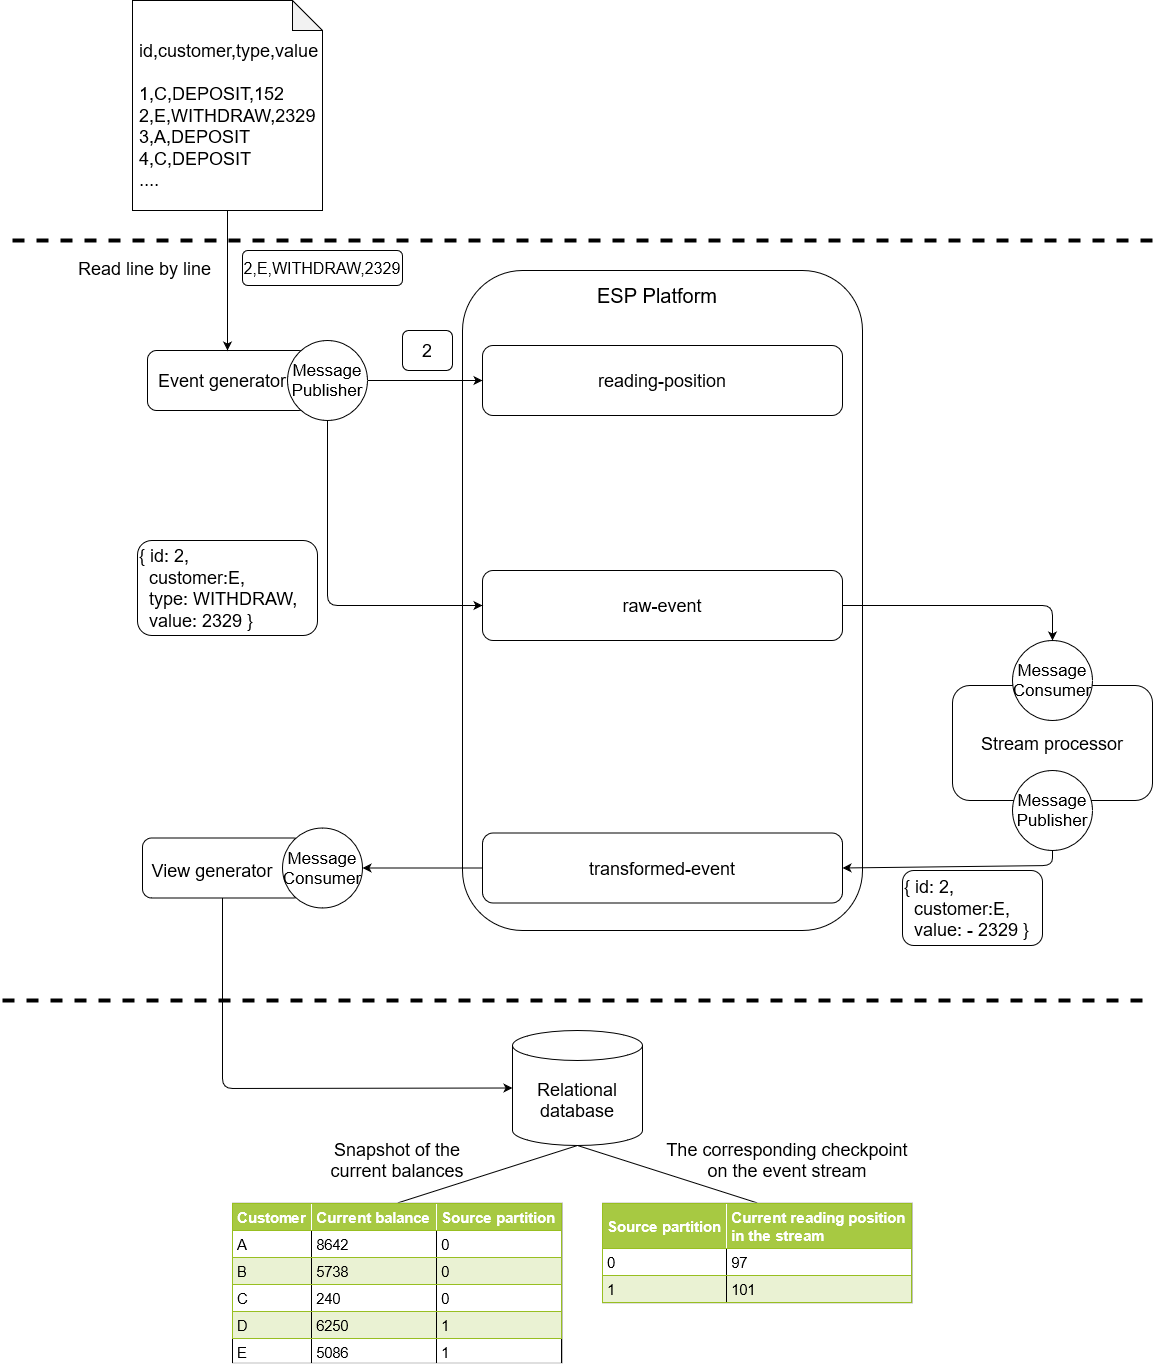
\includegraphics[width=18cm,height=\textheight]{images/implementation-use-case-1.png}
	\caption{Use case to implement delivery guarantee on the platforms.}
	\label{fig:impusecase}
\end{adjustwidth}
\end{figure}


Finally at the end of the event streams pipeline, the view generator component will accumulate the transactional values of each user and persist the resulted current balance to a relational database. In addition, the view generator also commit the corresponding reading position on the source stream \emph{Transformed event} to the database so that it can fetch this value and resume the consumption on the stream accordingly upon restarting.


With this setup, message duplication can be easily detected because any transactional event which is processed more than once by any of the three processing components will result in different final current balances. To verify that the configuration and implementation is correct on each platform to achieve the highest message delivery guarantee, different failure scenarios are setup. The final current balances in these scenarios will be verified against the result from a scenario without failure.

 
\subsection{Failure scenarios}
All three components: event generator, stream processor, and view generator have the processing cycle of an event as read-modify-write. After writing the modified event, these components must update the reading position on the source system to continue to receive subsequent events when they are restarted. Failure before updating reading position can lead to message duplication. As a result, three failure scenarios are derived for three processing components where they are simulated to be crashed before being able to checkpoint the reading position on the data source. 

For Apache Kafka and Apache Pulsar, another failure scenario is setup. Kafka and Pulsar support using the consumer group pattern to read a partitioned topic with multiple concurrent consumer instances (section \ref{section:patterns}). In this case, users have the option to rely on the failover mechanism of the consumer group to automatically manage and assign partitions of the topic to consumer instances in the same group. However, this can lead to the case same messages are sent and buffered on two different consumer instances when the platform transfer ownership of a partition from one consumer to another.

